\documentclass[10pt]{article}
\usepackage{icmlko}

\icmlmeta{IP 파운데이션 월드모델}{277}{챔피언의 맹점}{같은 열을 능형은 쓰고 나무는 못 쓴다 --- 정식화를 고르는 것이 어느 도메인의 말을 들을지 고르는 것이었다}

\begin{document}

\twocolumn[
\icmlheader

\begin{abstract}
노트 276이 규약 하나를 세웠다 --- ``학습행이 \texttt{2$\times$min\_samples\_leaf}
아래인 도메인에는 전용 이름을 주지 않는다.'' 근거는 나무의 분기 규칙이었다.
그러면 \textbf{분기가 없는 정식화는 어떤가.} F21 능형에는 잎 하한이 없다.
같은 열을 그대로 줘 봤다. \textbf{능형은 배운다} --- 팝업에 라벨 순위를
전용 열로 주면 $+$0.0880 이고, 나무는 \textbf{정확히 $+$0.0000} 이다.
\textbf{벽은 자료가 아니라 정식화에 있었다.} 그래서 노트 276의 규약에
범위를 단다 --- \textbf{나무 계열에서만}이다. 그런데 같은 실험이 팝업 전용
축 갈래를 \emph{두 번째로} 닫는다: \textbf{진짜 축 넷은 능형에서도 안 된다}
($-$0.0070). 배울 수 있는 자리에서도 안 배워지는 것이니 그 열들에 쓸 신호가
없는 것이다. 벽과 무신호는 따로다. 남는 것은 더 큰 이야기다 --- 챔피언
F18(나무)과 준우승 F21(능형)은 판 $\rho$ 로 0.4842 대 0.4544 인데, 그
차이 뒤에 \textbf{``작은 도메인의 전용 정보를 쓸 수 있는가''라는 갈림이
숨어 있다.} F18은 못 쓰고 F21은 쓴다. 판은 이 차이를 못 본다 --- 팝업이
2.3\% 라서다(노트 274). \textbf{정식화를 고르는 것이 어느 도메인의 말을
들을지 고르는 것이었고, 우리는 그걸 모르고 골랐다.}
\end{abstract}
]

\section{규약에 범위를 달아야 했다}

노트 276이 팝업 전용 축 넷의 $+$0.0000 을 파고들어 범인을 찾았다 ---
\texttt{HistGradientBoostingRegressor} 의 \texttt{min\_samples\_leaf} 기본값
20 이고, 팝업의 관측 학습행은 14다. 어느 쪽 잎도 20을 못 채우니 그 열로
가르는 분기가 후보에도 못 오른다.

그리고 규약을 적었다 --- 학습행이 \texttt{2$\times$}잎 하한 아래면 전용
이름을 주지 말고 공유 축에 태우라고. \textbf{그 규약은 나무를 보고 쓴
것이다.} 능형은 분기가 없고 계수를 푼다. 16행짜리 열에도 계수는 붙는다
(작게 붙을 뿐이다). \textbf{규약이 판 전체의 것인지 나무의 것인지 재야
했다.}

\section{능형은 배운다}

\begin{figure*}[t]
\centering
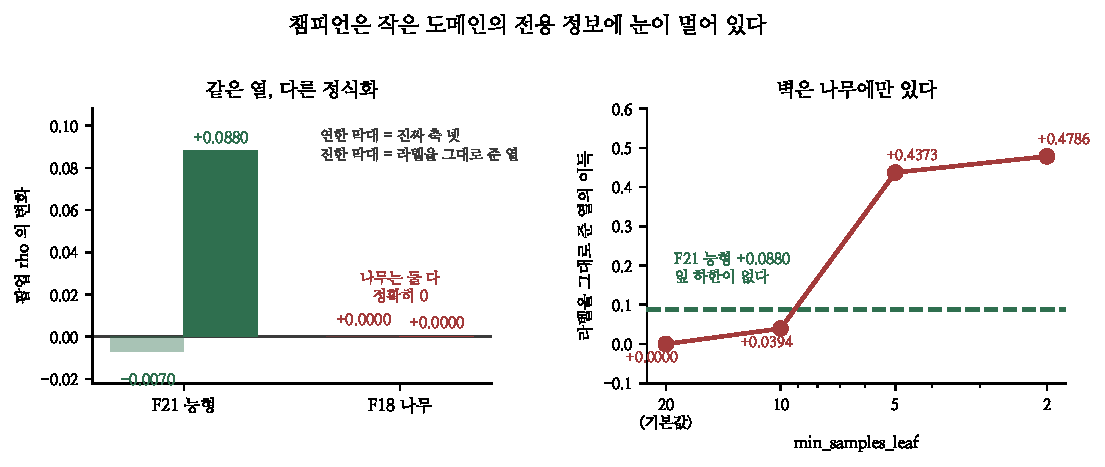
\includegraphics[width=\textwidth]{figs/blind.pdf}
\caption{왼쪽 --- 같은 열 둘(진짜 축 넷, 라벨을 그대로 준 열)을 두 정식화에
줬을 때 팝업 $\rho$ 의 변화. 오른쪽 --- 노트 276의 잎 하한 곡선 위에 능형을
가로선으로 얹은 것. 능형은 잎 하한이라는 손잡이 자체가 없다.}
\end{figure*}

문턱 15 · 씨앗 0 으로 넷 칸을 다 쟀다.

\begin{center}\small
\begin{tabular}{llrrr}
\hline
정식화 & 준 열 & 팝업 전 & 팝업 후 & 차 \\
\hline
F21 능형 & 진짜 축 넷 & 0.3090 & 0.3020 & $-$0.0070 \\
F21 능형 & 라벨 누출 & 0.3090 & 0.3970 & \textbf{$+$0.0880} \\
F18 나무 & 진짜 축 넷 & 0.3819 & 0.3819 & $+$0.0000 \\
F18 나무 & 라벨 누출 & 0.3819 & 0.3819 & \textbf{$+$0.0000} \\
\hline
\end{tabular}
\end{center}

\textbf{능형은 14행짜리 전용 열을 읽는다.} 나무는 같은 열을 두 번 다
정확히 무시한다. \textbf{노트 276의 규약은 나무 계열에서만 산다.}

\paragraph{능형도 크게는 못 읽는다} $+$0.0880 은 라벨을 통째로 준 값이다.
큰 도메인들이 같은 대접에서 받는 것은 $+$0.35$\sim$0.70 이고, 나무도 잎
하한을 5로 내리면 $+$0.4373 을 받는다. 능형이 14행에서 얻는 $+$0.0880 은
그 5분의 1 이다 --- L2 가 표본 적은 열의 계수를 세게 줄인다. \textbf{작은
도메인의 전용 열은 능형에서도 약하게만 산다.} 다만 \emph{0 은 아니다},
그리고 0 과 0.0880 사이가 이 노트의 전부다.

\section{그리고 갈래가 두 번째로 닫힌다}

같은 표의 첫 줄이 조용히 중요하다. \textbf{진짜 축 넷은 능형에서도
$-$0.0070 이다.} 능형은 그 열을 읽을 수 있는데도 이득이 없다.

\begin{center}\small
\begin{tabular}{ll}
\hline
왜 팝업 전용 축이 안 되나 & \\
\hline
나무에서 & \textbf{못 읽는다} (잎 하한 20 $>$ 14행) \\
능형에서 & \textbf{읽는데 쓸 게 없다} ($-$0.0070) \\
\hline
\end{tabular}
\end{center}

\textbf{둘은 다른 이유다.} 노트 276만 있었으면 ``손잡이만 풀면 된다''로
읽혔을 텐데, 능형이 그 해석을 막는다. \texttt{pop\_comp} ·
\texttt{pop\_wkend} · \texttt{pop\_holid} · \texttt{pop\_stores} 넷은 채택
검사 ①③ 을 통과했지만 \textbf{배울 수 있는 자리에서도 안 배워진다.}
채택 검사가 학습 구간 상관을 보는데 유보에서 안 나오는 것이니, 노트 256이
검사 셋을 세울 때 남긴 ``통과가 근거는 아니다''의 또 한 사례다.

\section{판이 못 보는 갈림}

여기서 남는 것이 제일 크다. 챔피언 F18(나무)과 준우승 F21(능형)은 지금
판에서 0.4842 대 0.4544 다. 노트 126의 동점 규칙과 노트 268의 재판정이
그 순서를 정했고, 그 결정은 \textbf{판 $\rho$ 하나로} 내려졌다.

그런데 오늘 잰 것은 판이 못 재는 축이다.

\begin{center}\small
\begin{tabular}{lcc}
\hline
& F18 나무 & F21 능형 \\
\hline
판 $\rho$ & \textbf{0.4842} & 0.4544 \\
작은 도메인 전용 정보 & \textbf{못 쓴다} & 쓴다 \\
\hline
\end{tabular}
\end{center}

판은 이 두 번째 줄을 못 본다 --- 팝업이 유보의 2.3\% 이고, 노트 274가 잰
대로 팝업에서 도메인 안 $\Delta\rho{=}0.435$ 가 있어야 판이 겨우 반응하기
때문이다. \textbf{그러니 챔피언을 고른 판정치는 이 성질에 대해 아무 말도
안 했다.} 우연히 그렇게 됐을 뿐이다.

이것이 노트 254 · 274 · 275가 세 번 짚은 것의 네 번째 얼굴이다. 앞의 셋은
``판정 단위와 배포 단위가 다르다''였는데, 이번 것은 한 겹 더 안쪽이다 ---
\textbf{판정치는 정식화의 어떤 성질을 고르는지 자기도 모른다.}

\paragraph{그래서 뒤집자는 게 아니다} F21로 갈아타자는 결론은 안 나온다.
$+$0.0880 은 라벨을 통째로 준 값이고 진짜 축에서는 $-$0.0070 이다 ---
\textbf{지금 팝업에 쓸 전용 정보 자체가 없다.} 바뀌는 것은 앞으로다:
\textbf{작은 도메인의 전용 정보를 쓰겠다고 정하는 순간, 정식화 선택이 그
결정의 일부가 된다.} 그때는 판 $\rho$ 가 그 선택을 대신 해 주지 않는다.

\paragraph{남은 것}
\begin{center}\small
\begin{tabular}{ll}
\hline
갈래 & 왜 \\
\hline
넷을 공유 축에 태우기 & 능형에서도 $-$0.0070 이라 기대는 낮다 \\
아이돌 54행 & 벼랑 바로 위. 전용 축이 실제로 될까 \\
정식화 성질표 & 판이 못 보는 성질을 따로 적어 둘 것 \\
잎 하한 정식 판정 & 노트 275 규칙 ②로. 판은 $-$0.0018 \\
\hline
\end{tabular}
\end{center}

\paragraph{규약} \textbf{규약을 세울 때 그 규약이 어느 정식화의 성질에서
나왔는지 적는다.} 노트 276의 규약은 하루도 안 돼 범위가 좁아졌다 --- 나무의
잎 하한에서 나온 것을 판 전체의 규칙처럼 썼다. 그리고 \textbf{판정치가 못
보는 성질은 판정치가 골라 주지 않는다} --- 그런 성질은 손으로 적어 두고
손으로 고른다.

\end{document}
